\documentclass[tikz,border=0cm,dvipsnames,x11names,rgb]{standalone}

\usepackage{amsmath,amssymb,amsfonts}
\usetikzlibrary{calc,
fit,
shapes.misc,
shapes.geometric,
arrows.meta,
fadings,
matrix,
chains,
scopes,
positioning}

\usepackage{pgfplots}
\usepackage{pgfplotstable}
\pgfplotsset{compat=1.18}



\usepackage[]{fontspec}

\setmainfont{Latin Modern Roman}
\setmonofont{Latin Modern Math}
\renewcommand{\textsc}[1]{{\fontfamily{lmr}\selectfont \scshape #1}}

\usepackage[]{bm}

\makeatletter
\@ifundefined{fromRoot}{\newcommand{\fromRoot}[1]{../../#1}}{}

\def\input@path{{../..}{..}{.}{./svg}{./pgfplots}{./tikzpicture}}
%or: \def\input@path{{/path/to/folder/}{/path/to/other/folder/}}
\makeatother

\newcommand{\ra}[1]{\renewcommand{\arraystretch}{#1}}

\newcommand*{\gf}[1]{\acrshort{gf}($#1$)}%
\newcommand*{\mpn}[1]{\bm{P}_{#1}}%
\newcommand*{\pn}[1]{%
  \ifthenelse{\equal{#1}{}}{$\mpn{0}$}{$\mpn{#1}$}%
}%

\newcommand*{\pk}[3]{%
  \ifthenelse{\equal{#1}{#2}}{\textcolor{red}{\phantom{.}$p_0$\phantom{.}}}{\phantom{.}$p_#3$\phantom{.}}%
}%


\newcommand*{\placeholderreg}{\includegraphics[width=\linewidth, height=.25\textheight, keepaspectratio = true]{figures/certified_xilinx.png}}%
\newcommand*{\placeholder}[1]{\includegraphics[#1]{figures/certified_xilinx.png}}%

\newcommand*{\snr}{\acrshort{snr}}%
\newcommand*{\snrs}{\acrshortpl{snr}}%

\newcommand*{\mpd}[0]{p_\Delta}%
\newcommand*{\mpo}[0]{p_\omega}%
\newcommand*{\pd}[0]{$\mpd$}%
\newcommand*{\po}[0]{$\mpo$}%
\newcommand*{\mpfa}[0]{\mathcal{P}_{fa}}%
\newcommand*{\mpmd}[0]{\mathcal{P}_{md}}%
\newcommand*{\pfa}[0]{\acrshort{pfa}}%
\newcommand*{\pmd}[0]{\acrshort{pmd}}%
\newcommand*{\mnorm}[1]{\mathcal{L}_{#1}}%
\newcommand*{\norm}[1]{$\mnorm{#1}$}%
\newcommand*{\fft}{\acrshort{fft}}%
\newcommand*{\mfft}[1]{\mathcal{F}(#1)}%
\newcommand*{\mifft}[1]{\mathcal{F}^{-1}(#1)}%
\newcommand*{\ts}{\acrshort{ts}}%

\newcommand*{\cpp}[1]{C\textrm{++#1}}%
\newcommand*{\na}{\textrm{\textcolor{SlateGray4}{N/A}}}%

\newcommand*{\vect}[1]{\bm{#1}}%
\newcommand*{\mat}[1]{\bm{\mathrm{#1}}}%

\newcommand*{\task}[1]{\mathcal{T}_{#1}}%

\newcommand*{\sdr}{\acrshort{sdr}}%
\newcommand*{\fpga}{\acrshort{fpga}}%

\newcommand*{\rikiki}{\fontsize{4}{6}\selectfont}%



\begin{document}

\pgfdeclarelayer{background}
\pgfsetlayers{background, main}
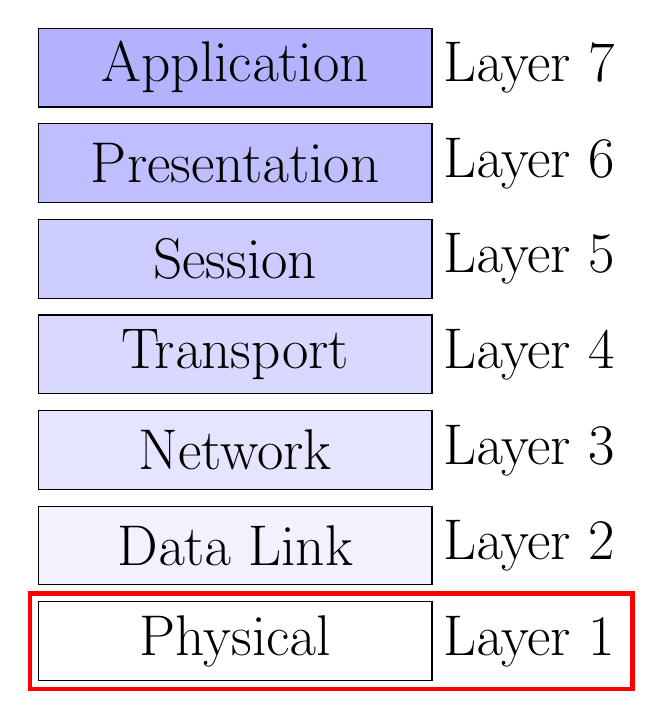
\begin{tikzpicture}[
  every node/.style={font=\huge}
]

  \node [
    draw,
    fill=blue!00,
    minimum width = 5cm,
    minimum height = 1cm] (lv1) at (0,0) {Physical};
  \node [
    draw,
    fill=blue!05,
    minimum width = 5cm,
    minimum height = 1cm,
    above = 2mm of lv1
  ] (lv2) {Data Link};
  \node [
    draw,
    fill=blue!10,
    minimum width = 5cm,
    minimum height = 1cm,
    above = 2mm of lv2
  ] (lv3) {Network};
  \node [
    draw,
    fill=blue!15,
    minimum width = 5cm,
    minimum height = 1cm,
    above = 2mm of lv3
  ] (lv4) {Transport};
  \node [
    draw,
    fill=blue!20,
    minimum width = 5cm,
    minimum height = 1cm,
    above = 2mm of lv4
  ] (lv5) {Session};
  \node [
    draw,
    fill=blue!25,
    minimum width = 5cm,
    minimum height = 1cm,
    above = 2mm of lv5
  ] (lv6) {Presentation};
  \node [
    draw,
    fill=blue!30,
    minimum width = 5cm,
    minimum height = 1cm,
    above = 2mm of lv6
  ] (lv7) {Application};

\foreach \i in {1,2,3,4,5,6,7} {
  \node [right = .1mm of lv\i] (lv\i_lb) {Layer \i}; 
}

\node [draw=red, ultra thick, inner sep=1mm, fit = (lv1) (lv1_lb) ] {};

\end{tikzpicture}
\end{document}

